\chapter{Resumen Extendido}

La edad de las estrellas es una de las propiedades más difíciles de medir, ya que no puede observarse de forma directa, y a su vez, es algo fundamental para profundizar en otros problemas astrofísicos, como la búsqueda de vida fuera del sistema solar. Entre las técnicas disponibles para abordar esta tarea se encuentra la girocronología, que permite estimar las edades estelares mediante el periodo de rotación de las estrellas.

Las estrellas nacen con una determinada velocidad de rotación y sufren una reducción de esta velocidad por el proceso de frenado magnético. Se sabe que cuanto mayor sea la rotación, mayor será su frenado, y por lo tanto, todas las estrellas tienden a converger a una velocidad de rotación similar para una edad y masa concreta. Es la girocronología la técnica que explota este hecho.

Esta prometedora técnica presenta una gran ventaja frente a otras, que consiste en la facilidad para obtener entradas de observación a analizar. Aunque, por otro lado, existen una serie de incertidumbres que la convierten en una técnica de estimación de edades estelares poco precisa, además de presentar limitaciones en cuanto al rango de masa de las estrellas sobre las que se puede aplicar esta técnica.

\vspace{0.5cm}

Teniendo esto en cuenta, se propone explorar el problema de la datación estelar utilizando la girocronología desde la perspectiva de la Inteligencia Artificial. La idea consiste en reemplazar las combinaciones lineales y las técnicas tradicionales que se emplean en la girocronología convencional por una aproximación de regresión de aprendizaje automático.

Hasta el momento, existen pocos trabajos que aborden la datación de estrellas mediante técnicas de Inteligencia Artificial. Por ejemplo, en \cite{sanders2018}, se presenta por primera vez una Red Neuronal Bayesiana aplicada a la estimación de la edad de las estrellas. 

En este trabajo se propone un enfoque diferente al que han seguido otros autores en sus estudios, más detallados en la Sección \ref{sec:related_work}, ya que los modelos anteriores abordan el problema desde la perspectiva bayesiana. En cambio, aquí se propone un problema de regresión puro, donde los diferentes modelos estudiados se enfrentan a la estimación de un valor particular para la edad y se evalúan en consecuencia.

\vspace{0.5cm}
%TODO_DONE: No utilices palabras en inglés si hay una alternativa en castellano (dataset = conjunto de datos). Revisa todo el documento para que esto no se produzca en general.
La base de datos principal de este trabajo se compone de 1464 estrellas. Este conjunto de datos contiene varias características de cada una de las estrellas, tomando especial importancia: la temperatura efectiva $T_\texttt{eff}$, el logaritmo de la gravedad superficial $log$g, la masa estelar $M$, el radio estelar $R$, la metalicidad ${\rm [Fe/H]}$, el periodo de rotación $P_{\rm rot}$ y la edad a estimar. Estas edades precisas provienen de la astrosismología y de la pertenencia a cúmulos. Las 4 edades principales de los cúmulos son: 0.79, 1, 2.5 y 4.2 Gyrs.

Para seleccionar las estrellas que alimentarán los modelos en la fase de entrenamiento, validación y test, se realiza un filtrado previo sobre la base de datos comentada. En ella se seleccionan las estrellas FGK (estrellas de clases espectrales medias) y con periodo de rotación inferior a 50 días. El motivo de este filtrado se explica mediante la física que hay detrás de la girocronología, ya que ésta se ve limitada en un rango de masa de entre 0.7 y 2, y los periodos de rotación superiores a 50 días presentan dificultades a la hora de explicarse con la estructura estelar actual.

Es necesario añadir que esta muestra exhibe dos sesgos importantes: 1) la muestra perteneciente a la astrosismología está sesgada hacia las estrellas masivas y viejas; y 2) la muestra basada en cúmulos está sesgada hacia edades más jóvenes.

\vspace{0.5cm}

Los modelos que se han alimentado con esta muestra están detallados en la Sección \ref{sec:models} y son: Linear Regressor, Bayesian Regression, Decision Tree Regressor, Random Forest Regressor, Support Vector Regression, Gaussian Process, kNN, Neural Network y Stacking, siendo este último un método de ensamblado de modelos formado por Neural Network y Gaussian Process en el nivel 0 y por Linear Regressor en el nivel 1. La Red Neuronal empleada es un perceptron multicapa, está formada por 3 capas ocultas \emph{fully-connected} con 50 unidades en cada una de ellas.

El estudio de rendimiento de los modelos y su correspondiente comparativa se lleva a cabo mediante tres \emph{benchmarks}. En estos, se proponen tres escenarios de evaluación con el fin de evaluar diferentes capacidades mediante el error medio absoluto (MAE) de los modelos. El MAE permite cuantificar la precisión de las estimaciones de edad comparando el valor predicho frente al observado.

\vspace{0.25cm}
%TODO_DONE: explica que es el MAE antes de nombrarlo
\textbf{Problema de datación estelar (Benchmark A)} {} Configuración para evaluar los modelos de regresión bajo un esquema clásico de división de datos en entrenamiento y prueba, siguiendo una distribución de 80\%/20\% respectivamente. En este escenario, los modelos que mejor rendimiento muestran son Neural Network, Gaussian Process y su Satcking, presentando un MAE inferior a 0.46 Gyrs, tal y como se puede apreciar en la Figura \ref{fig:benchA_models_intro}.

\begin{figure}[H]
\begin{center}
 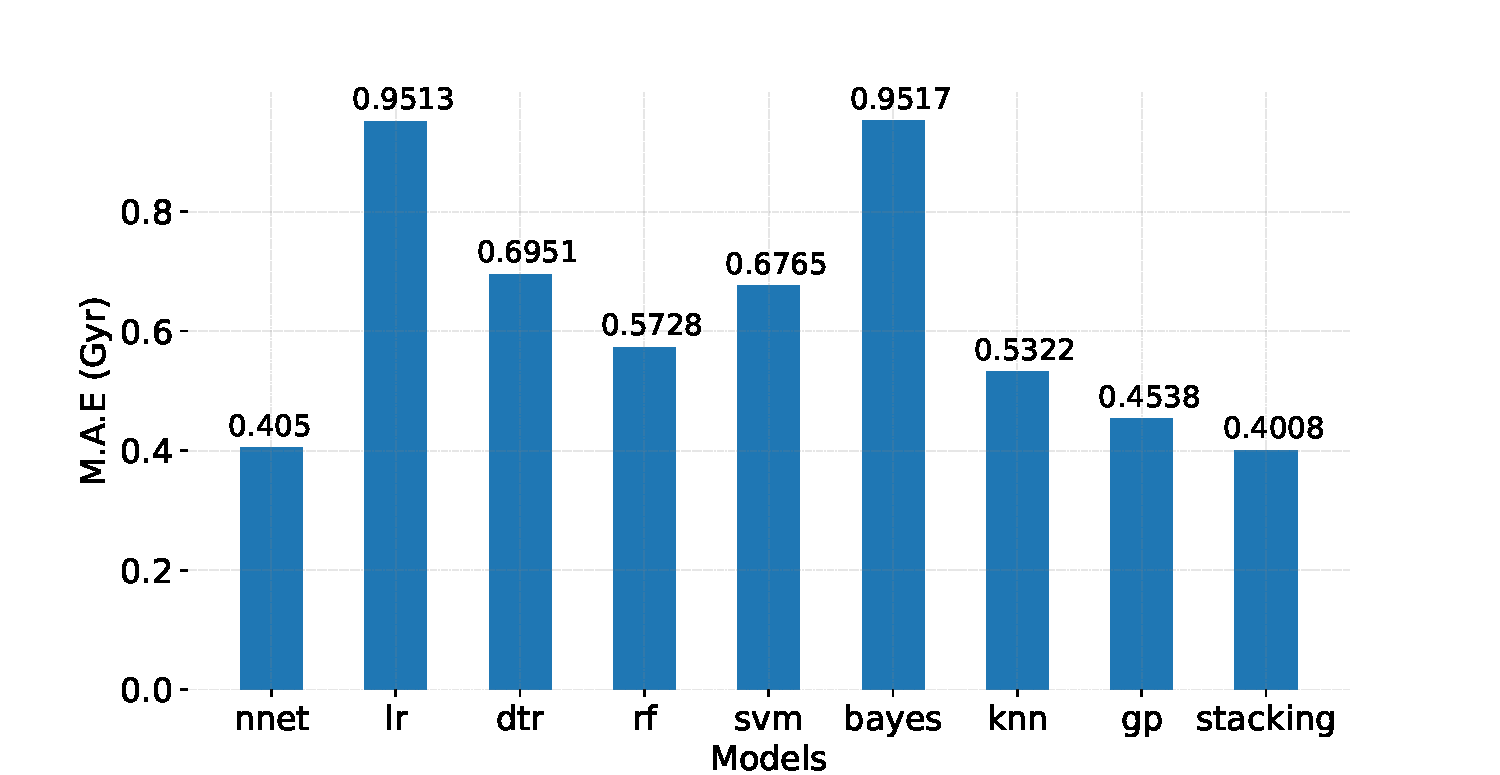
\includegraphics[width=0.8\linewidth]{Figuras/Experimentos/B_A_models.pdf}
\end{center}
\caption{Benchmark A: Rendimiento de los modelos en función del MAE. En esta configuración, las dos mejores aproximaciones son Neural Network (nnet) y Gaussian Process (gp), y por lo tanto, su Stacking.}
 \label{fig:benchA_models_intro}
\end{figure}

\vspace{0.25cm}

\textbf{Capacidad de generalización (Benchmark B)} {} Este Benchmark se compone de dos configuraciones diferentes: 1) Benchmark B1, donde se evalúa la capacidad de los modelos para estimar edades de estrellas cuyo rango está fuera del de las estrellas vistas durante el entrenamiento; y 2) Benchmark B2, en el que se evalúa la capacidad de generalización entrenando los modelos con las estrellas pertenecientes a cúmulos y probando con el resto de estrellas. Los resultados de los modelos para estos dos escenarios muestran peor MAE que para el Benchmark A, concluyendo que todos los modelos presentan dificultades a la hora de generalizar. Para la configuración del Benchmark B1, el modelo que mejor resultado presenta es el de Neural Network, mientras que para el Benchmark B2 es uno de los modelos que peor rendimiento muestra, siendo Bayesian Regression el que mejor resultado devuelve en este escenario. Ver Figura \ref{fig:benchB1_intro} y Figura \ref{fig:benchB2_intro} para visualizar todos los rendimientos.
%TODO_DONE: ojo, todas las figuras que menciones deben aparecer aquí repetidas, pues este resumen debe ser autocontenido.

\begin{figure}[H]
\begin{center}
 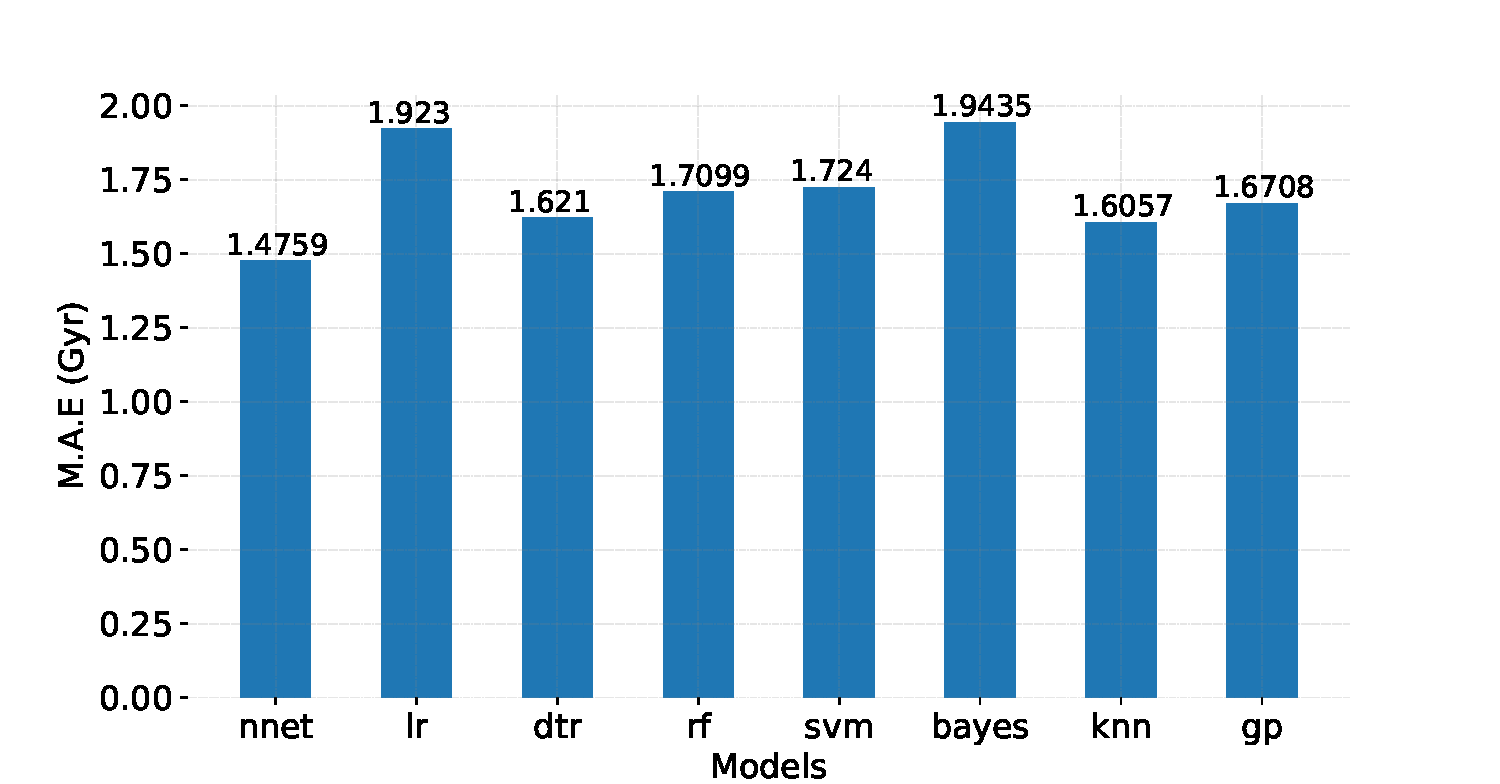
\includegraphics[width=0.8\linewidth]{Figuras/Experimentos/B_B1_models.pdf}
\end{center}
\caption{Benchmark B1: Rendimiento de los modelos en función del MAE.}
 \label{fig:benchB1_intro}
\end{figure}

\begin{figure}[H]
\begin{center}
 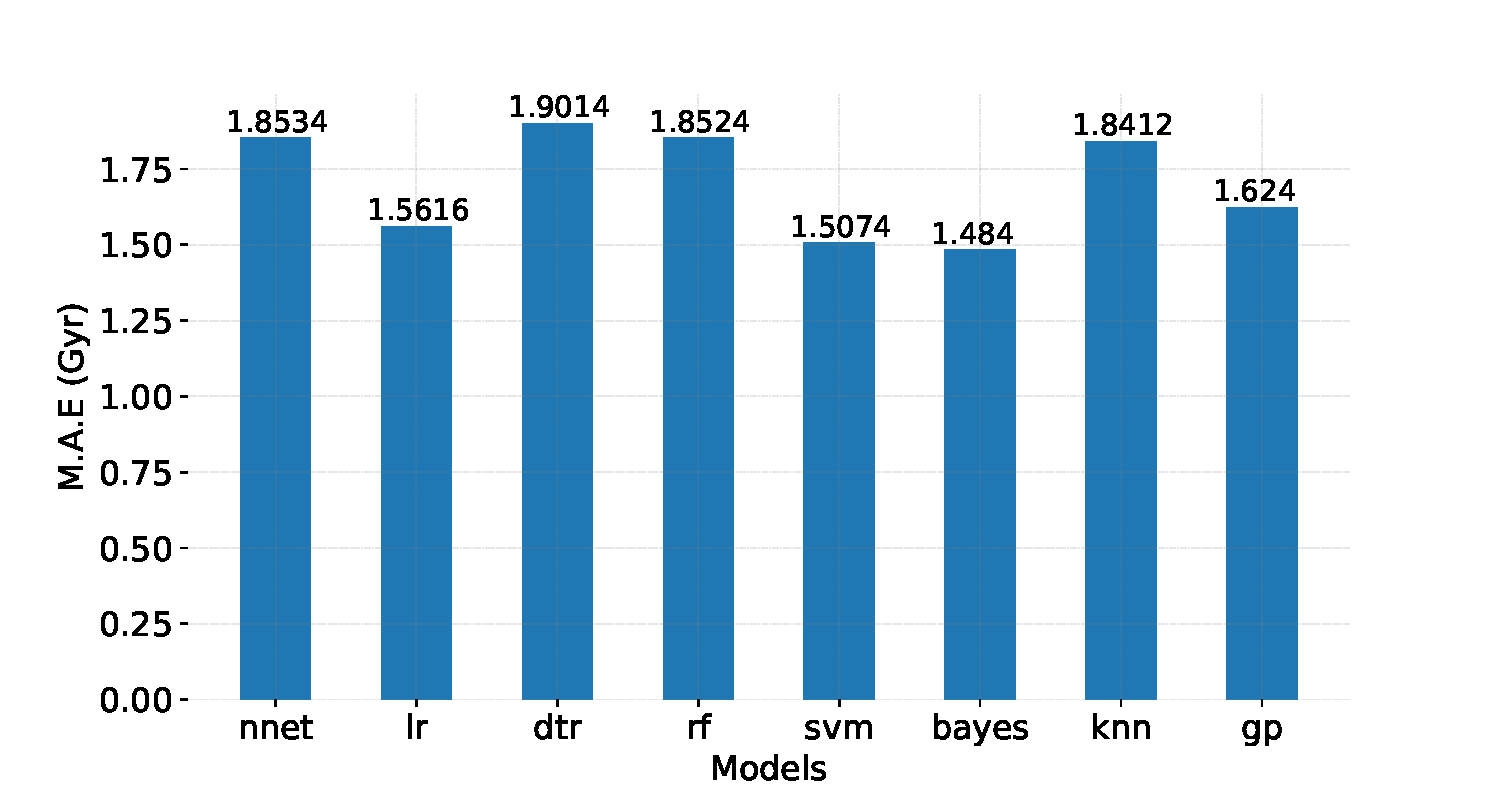
\includegraphics[width=0.8\linewidth]{Figuras/Experimentos/B_B2_models.pdf}
\end{center}
\caption{Benchmark B2: Rendimiento de los modelos en función del MAE.}
 \label{fig:benchB2_intro}
\end{figure}

\vspace{0.25cm}

\textbf{Regresión sobre una muestra de control (Benchmark C)} {} En este último escenario se evalúan los modelos sobre una muestra de control de 32 estrellas, extraídas del conjunto de datos filtrado y desconocidas en todos los entrenamientos realizados. Entre estas 32 estrellas se encuentra el Sol, haciéndose énfasis en la estimación de su edad. En esta ocasión, los tres mejores modelos son Gaussian Process, Neural Network y su Stacking. La Figura \ref{fig:benchC_intro} muestra el MAE para cada modelo. En cuanto a la estimación de la edad del Sol, tal y como se puede observar en la Tabla \ref{table:sun_results_intro}, el modelo que más se aproxima a los 4.6 Gyrs es Random Forest Regressor, estimando una edad de 4.76 Gyrs.

\begin{figure}[H]
\begin{center}
 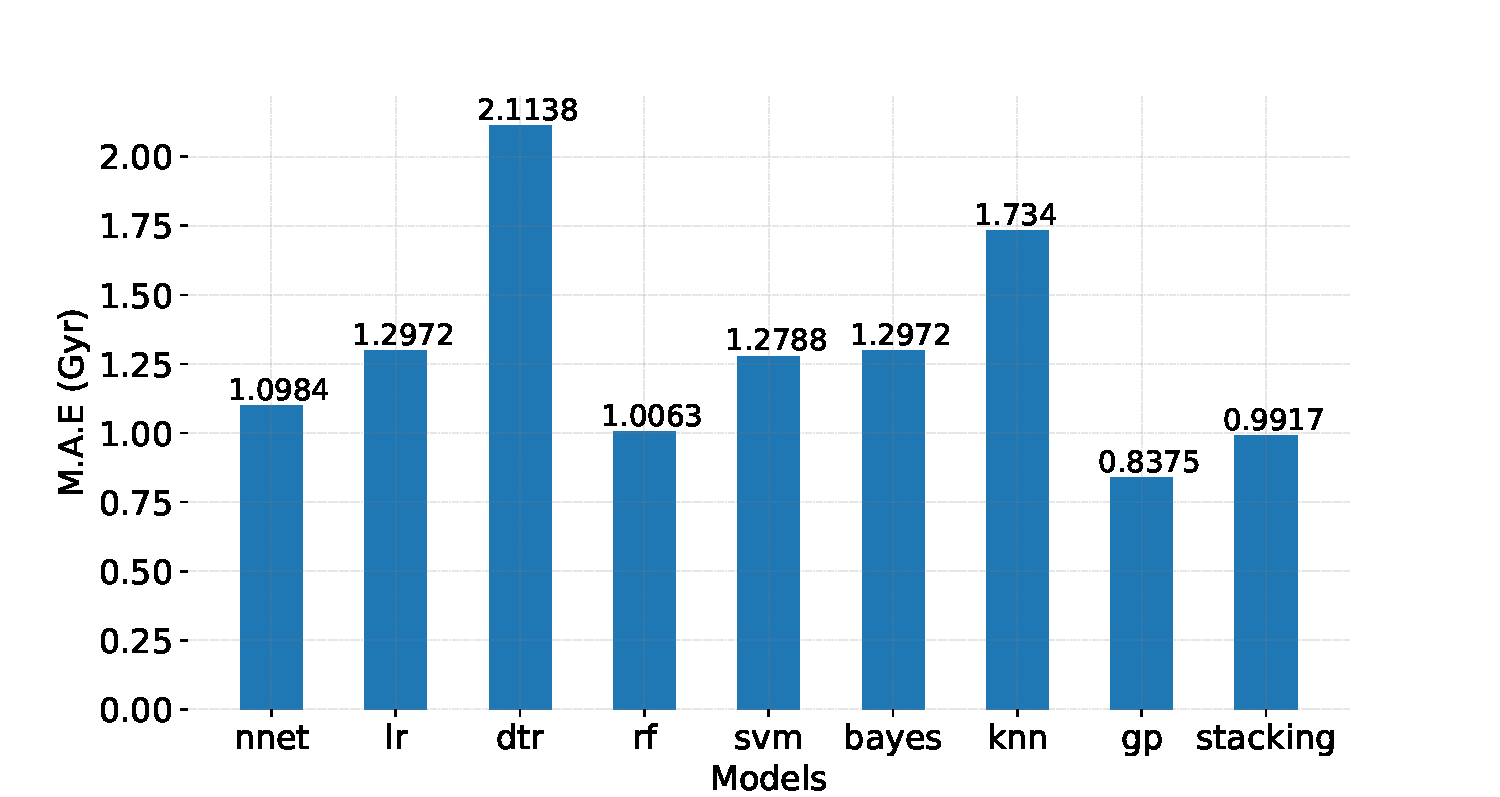
\includegraphics[width=0.8\linewidth]{Figuras/Experimentos/B_C_models.pdf}
\end{center}
\caption{Benchmark C: Rendimiento de los modelos en función del MAE.}
 \label{fig:benchC_intro}
\end{figure}

\begin{table}[H]
\centering
\scalebox{0.6}{
\begin{tabular}{l|ccccccccc}  
\toprule
\textbf{Modelos}  & nnet & lr & dtr & rf & svm & bayes & knn & gp & stacking \\
\midrule
Sol (4.6 Gyr)  & 4.02 & 3.92 & 4.49 & 4.76 & 3.81 & 3.91 & 4.49 & 3.88 & 4.02\\
\bottomrule
\end{tabular}
}%end of scalebox
\caption{Edad estimada para el Sol en Gyr. El método más preciso es rf. }\label{table:sun_results_intro}
\end{table}

\vspace{0.5cm}

Se obtienen tres conclusiones claras tras el estudio: 1) el modelo de Neural Network proporciona buenos resultados en 3 de los 4 escenarios evaluados, pudiendo asignarle el título simbólico de ganador; 2) todos los modelos tienden a subestimar, por lo que se cree que sería interesante tratar de corregir este sesgo en futuras líneas de investigación; y 3) el estudio revela resultados prometedores, obteniendo MAEs inferiores a 0.5 Gyrs, pudiendo considerarse como gran avance en el campo de la datación de estrellas.

\vspace{0.25cm}
%TODO_DONE: Motiva el empleo de meta-learing (aprender a parender con pocas muestras), y la utilidad que puede tener en el problema de la datación estelar.
Además del \emph{benchmarking} de los modelos clásicos de Inteligencia Artificial, se realiza un estudio sobre la aplicación del algoritmo MAML (\emph{Model-Agnostic Meta-Learning}) \cite{finn2017modelagnostic} para el problema de estimación de edades estelares. Este algoritmo se denomina agnóstico del modelo porque es compatible con cualquier algoritmo entrenado con descenso de gradiente. Y se caracteriza por el metaaprendizaje porque se entrena en varias tareas de aprendizaje con el objetivo de que sea capaz de resolver nuevas tareas con una pequeña cantidad de muestras.

\vspace{0.25cm}
La motivación principal para usar este tipo de algoritmos se basa en su capacidad de aprendizaje con pocas muestras, esto es útil cuando se trabaja con conjuntos de datos reducidos. Este es uno de los aspectos principales por los que aplicar este tipo de algoritmos sobre el problema de datación estelar. Además de que se parte de un conjunto de datos relativamente reducido, con el paso del tiempo se obtendrán de conjuntos de datos muy reducidos, provenientes de diferentes fuentes y misiones espaciales. Este tipo de algoritmos facilitan el uso de estos conjuntos reducidos para reforzar los modelos probados con estrellas anteriores.  

%TODO_DONE: revisa la última frase, pues no entiendo lo que quieres decir con "para el metaaprendizaje"

\vspace{0.25cm} 

Durante la fase de metaentrenamiento, el modelo se entrena para que sea capaz de adaptarse a un número muy elevado de tareas, todas con pocas muestras. Esto se consigue mediante la configuración de aprendizaje tipo \emph{K-Shot}, donde el modelo se entrena para que aprenda nuevas tareas usando K muestras de la observación inicial y la retroalimentación proporcionada por la función de pérdidas para cada tarea. El ajuste del modelo sigue una regla de aprendizaje basada en gradientes, con el objetivo de aprender rápidamente sobre nuevas tareas extraídas de la distribución total sin llegar al sobreajuste. 

\vspace{0.25cm}

El funcionamiento detallado del algoritmo y la inyección de los datos relativos a las características de las estrellas se explican en la Sección \ref{sec:maml}. Para evaluar los resultados obtenidos de este experimento, se emplea la misma métrica que se utiliza en el trabajo original \cite{finn2017modelagnostic}, el error cuadrático medio entre la edad estelar estimada y la edad estelar real. En este cálculo se tienen en cuenta los errores obtenidos en todos los pasos de actualización de gradiente, por lo que, el error cuadrático medio final se obtienen haciendo la media de todos estos.   %TODO_DONE: Detalla enter qué
Esta evaluación se realiza sobre distintas arquitecturas que pueden componer la red neuronal principal del modelo. Originalmente, se desarrolla con una red neuronal de 2 capas ocultas y 40 unidades cada una, pero los mejores resultados obtenidos se consiguen con una arquitectura de 3 capas ocultas y 20 unidades cada una, obteniendo un MSE = 0.01 en sus últimas actualizaciones de gradiente.

%TODO_DONE: Cierra resumiendo las conclusiones principales del TFM
Tras analizar los métodos clásicos y el algoritmo MAML se concluye que los resultados obtenidos en ambos experimentos son muy prometedores para el campo de la estimación de edades estelares. En el análisis de modelos clásicos destaca el modelo de la red neuronal, que funciona notablemente en 3 de los 4 escenarios propuestos, aunque se demuestre que todos los modelos tienden a subestimar. Respecto al algoritmo MAML, destaca una configuración de red de 3 capas ocultas con 20 unidades cada una, lo que permite obtener valores de MSE cercanos a 0 en la última actualización de gradiente. Además, se cree conveniente el uso de otros algoritmos de metaaprendizaje que permitan comparar sus resultados con los obtenidos por el algoritmo MAML.
